\chapter{Introduction}

NAND flash storage devices are widely used in both embedded and server applications. The research results from the related fields, such as~\cite{Chang:2010}, \cite{Wu:2010}, and \cite{Chang:2012}, have helped to fuel the continuous improvements to the design and performance of NAND flash storage devices. Other types of non-volatile storage devices, such as PCM (Phase-Change Memory)~\cite{Zilberberg:2013}, MRAM (Magnetoresistive RAM), and FeRAM (Ferroelectric RAM)~\cite{Doh:2007}, are also being actively studied. Recently in 2015, Intel Corp. and Micron Technology Inc. have launched a new class of non-volatile memory called 3D Xpoint~\cite{wiki:3DXpoint}. 3D Xpoint has a stackable and transistor-less design, and it is claimed to have the potential of being up to 1,000 times faster than NAND flash and 8 to 10 times denser than DRAM. Therefore, it can be expected that there will be an ever increasing number of storage elements to choose from for building storage subsystems.

From a system-level perspective, a storage subsystem is consists of the physical storage device hardware and the software modules in the OS that control how the storage hardware is utilized. In particular, the software modules can include components such as the file-system layer, I/O scheduler, volume manager, block device driver, etc. The storage subsystem is driven by I/O workloads generated by application programs and activities internal to the OS, such as demand paging and memory swapping.

The design and characteristic of storage subsystems can have great influences in determine the overall system performance and end user experience in many scenarios~\cite{Kim:2012}. Benchmarking a storage component in isolation or with overly simplified system-level models can result in inaccurate performance evaluations. While theoretical analysis or simulation using abstract models can provide quick estimates on how different storage subsystems might affect the overall system performance, the accuracy of these approaches can be rough and can therefore lead to design conclusions that are contradictory to the real-world results~\cite{Thekkath:1994}. It has been shown that when simulating using abstract models, complex system-level interactions can hide or reduce the predicted effects of new storage subsystem designs~\cite{Ganger:1998}.

As illustrated in Figure~\ref{fig:full-system workload}, when designing storage subsystems, it is desirable that the engineers will be able to evaluate the design choices with the overall system-level behaviors in mind. For example, computer system architects might want to know how storage subsystem of different characteristics will affect the overall system performance. For storage device designers, it would be desirable that they can test simulated storage devices that are not yet available with realistic workloads so that early stage design trade-offs can be made with the overall performance in mind.

\begin{figure}[htpb]
	\centering
	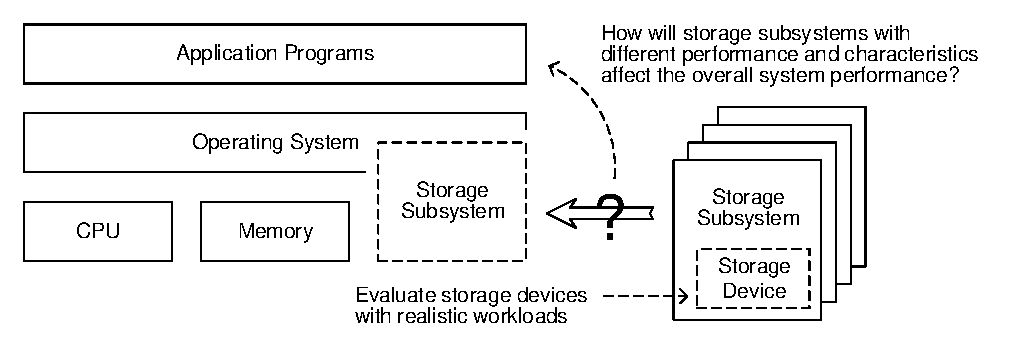
\includegraphics[width=\textwidth]{figures/Full-system.pdf}
	\caption[Evaluating storage subsystems in full-system context.]{\label{fig:full-system workload}The behaviors of the OS and application programs should be considered when trying to evaluate storage subsystems and storage devices.}
\end{figure}

When benchmarking storage subsystems, being able to use the real OS and application programs for generating the workloads can help in considering as much of the system-level behaviors as possible. Furthermore, since the instruction codes of the OS and application programs are run by the CPU, there are never truly pure I/O-bound workloads. For example, a workload that is perceived as I/O-bounded when executing on a faster computer can become CPU-bounded when being run on a computer with a slower CPU. That is, the speed of the hardware which the  OS and application programs run on can also affect the benchmarking results. Therefore, depending on the accuracy required for the performance predictions, the behaviors of the underlaying hardware, such as the CPU and memory subsystems, should also be considered in enough detail.

\section{The Problem and Motivation}

The problem that this dissertation sets to solve is to provide a full-system performance evaluation environment that can be used to experiment with prototype storage devices. while accurately taking into account the system-level behaviors of a computer system. Ideally, the full-system performance evaluation environment should consider as much of the system-level behaviors as possible, such as the behaviors of the OS, the benchmarking applications, and the performance of the underlying hardware that runs the software.

One of the conventional approaches that permits system-level evaluation of prototype storage device is storage device emulation. In this approach, a prototype storage device is constructed and made available to the OS of the target computer system. To the OS, the prototype storage device can be interactive with just like a real storage device. Because the OS and application programs are run on the real hardware, the detailed behaviors of the hardware of the target system are automatically considered. One limitation of the storage device emulation approach is that because the storage device emulator needs to reply the I/O requests back to the OS in real-time, there exists a hard time limit on the amount of time that is permitted for simulating the response for each I/O request. The time limit is equal to the intended response time of each I/O request. If the storage device emulator cannot complete the processing of an I/O request in this time limit, then the OS will perceive a storage device that is slower than intended. Therefore, it can sometimes be challenging or even impossible to emulate faster storage devices.

Complete machine simulation is another approach that allows the evaluation of prototype storage devices in full-system contexts. In complete machine simulation, a detailed simulation model of the target computer hardware, including the virtual storage device, is constructed and simulated in the discrete-time domain. The simulation model is detailed enough to run the real OS and application programs and should have execution timings close to the hardware of the target system. Since everything is simulated in the discrete-time domain, the speed of the storage device that can be modeled will not be constraint by the speed of the simulation host. That is, storage device of any speed can be studied with the complete machine simulation approach. However, one problem with this approach is that it can take great amount of effort for constructing and validating the detailed complete machine simulation model. Furthermore, depending on the complexity of the simulation model the simulation speed can be orders of magnitude slower than the real hardware. 

The observation and motivation of this dissertation is that the real hardware of the target computer system already encompasses the most truthful model of the desired complete machine behaviors, if the real hardware can be used as part of the complete machine simulation model for performing full-system performance evaluations, then the efforts needed for constructing and validating the simulation model of the target computer hardware can be avoided. In addition, executing the OS and application programs on the real hardware will be much faster than running them on virtually simulated hardware models.

\section{Thesis Statement}

This dissertation proposes a novel OS state pausing methodology for permitting the co-simulation of virtually simulated storage devices with the real OS and application programs running on real computer hardware. By utilizing the proposed methodology to perform full-system performance evaluations, the detailed simulation model of the target computer hardware does not need to be constructed. Furthermore, because the co-simulation is performed in the discrete-time domain, the speed of the virtual storage device that can be simulated will not be limited by the performance of the available hardware.

\section{Overview of the Dissertation}

When evaluating storage subsystems, the workloads and metrics used are important to the quality of the performance prediction results. Ideally, the storage subsystem should be evaluated in a full-system context which takes into account the detailed behaviors of the OS, the application programs, and the underlying hardware that runs the software.

Several approaches that are conventionally used by engineers and researchers for evaluating storage subsystems are discussed. The approaches that are discussed includes: (1) benchmarking with I/O traces, (2) complete machine simulation, and (3) storage device emulation. The shortcomings of these approaches are also discussed.

This dissertation proposes a novel way of pausing the state of the OS that is running on real hardware so that the OS and application programs can be co-simulated with virtually simulated storage devices in the discrete-time domain. The state of the OS can be considered to be the combined state of all the processes running in the OS and the timer and counter values observed by the OS. By freezing the execution of all the processes running in the OS and the advancement of the timer and counter hardware, the state of the OS can be paused. By carefully synchronize the state progression of the OS with the virtually simulated storage device, a full-system co-simulation environment can be constructed.

In this dissertation, the proposed OS state pausing methodology for co-simulating virtual storage device and real computer system is utilized in two usage scenarios:

\begin{enumerate}
	
	\item In the first usage scenario, a full-system co-simulation environment is built by using the proposed OS state pausing methodology to perform co-simulation of simulated virtual storage device with the OS and application programs running on real computer hardware. The full-system co-simulator allows the simulated storage device to be evaluated using realistic workloads generated by real OS and application programs. Higher level metrics such as elapsed user time and quality of service (QoS) at the application level can be used to benchmark the storage subsystem. By fast-forward the simulation time when the entire system is doing noting but waits in the CPU idle loop for the next event to arrive, the proposed full-system co-simulator can achieve faster than real-time simulations. The proposed full-system co-simulator has demonstrated up to 45$\times$ faster than real-time simulation speed in the experimental setup.
	
	\item In the second usage scenario, a storage device emulator based on the proposed OS state pausing approach is implemented for the Linux OS on the ZedBoard platform.
		
	In the proposed storage device emulator, a virtual storage device is emulated and made available to the OS at the block device driver level. The state of the OS is paused whenever the storage device emulator is busy processing I/O requests from the OS. Because of the pause made to the OS state, the storage device emulator can take as long as it needs for preparing each I/O response without affecting the perceived I/O response time by the OS. This allows prototype storage devices of any speed to be made available to the OS for full-system performance evaluation without being constraint by the speed of the hardware used for emulating the storage device.
	
	The proposed emulator allows the researchers to be able to predict the overall system performance of a particular embedded system, in the case of this dissertation, the ZedBoard platform, when different storage devices are used. The accuracy of the proposed storage device emulator is compared to a RAMDISK based reference system. The evaluation results from the proposed storage device emulator are shown to be within 2\% differences to the reference system.
	
	The storage device emulator takes a two part design. The work of simulation of the storage device model and persistence of the actual data is offloaded to another computer as to minimize the impact on the target system that the storage device is to be emulated. In particular, the size of the simulated storage device is not limited by the available storage space on the target system.

\end{enumerate}

\section {Contributions}

This dissertation makes three main contributions:

\begin{enumerate}
	\item An OS state pausing methodology is proposed that allows virtually simulated virtual storage devices to be co-simulated with real OS and application programs running on real computer hardware.
	
	\item A full-system co-simulator based on the proposed virtual storage device and real computer system co-simulation methodology is built and discussed in detail. The full-system co-simulator can be used for evaluating storage subsystem designs using realist workloads and system-level metrics.
	
	\item A storage device emulator is built using the proposed virtual storage device and real computer system co-simulation methodology~\cite{Wu:2015}. The target system is the ZedBoard platform running the Linux OS. The proposed storage device emulator allows the the prediction of the overall system performance of the target system when different storage devices are available. The full source code of the proposed storage device emulator is made available to the public domain\footnote{\url{http://www.cs.nctu.edu.tw/~cjtsai/research/nctusde}}.
	 
\end{enumerate}

\section {The Organization}

The remainder of the dissertation is organized as follows. Chapter~\ref{ch:2} discusses several approaches that are conventionally used for evaluating storage subsystems designs. Previous works related to storage subsystem performance evaluation are also discussed. Chapter~\ref{ch:3} introduces the concept of OS state pausing and how it is used in the co-simulation of virtually simulated storage device and real computer system. Chapter~\ref{ch:5} describes a full-system co-simulator based on the OS state pausing co-simulation approach. Chapter~\ref{ch:6} describes a storage device emulator based on the OS state pausing co-simulation approach. Chapter~\ref{ch:7} summarizes the contributions of this dissertation and suggests some directions for future research.
